\section{Apéndices}

\subsection{Gráficas de Apoyo para la Arquitectura MVC}
\begin{figure}[h]
\centering
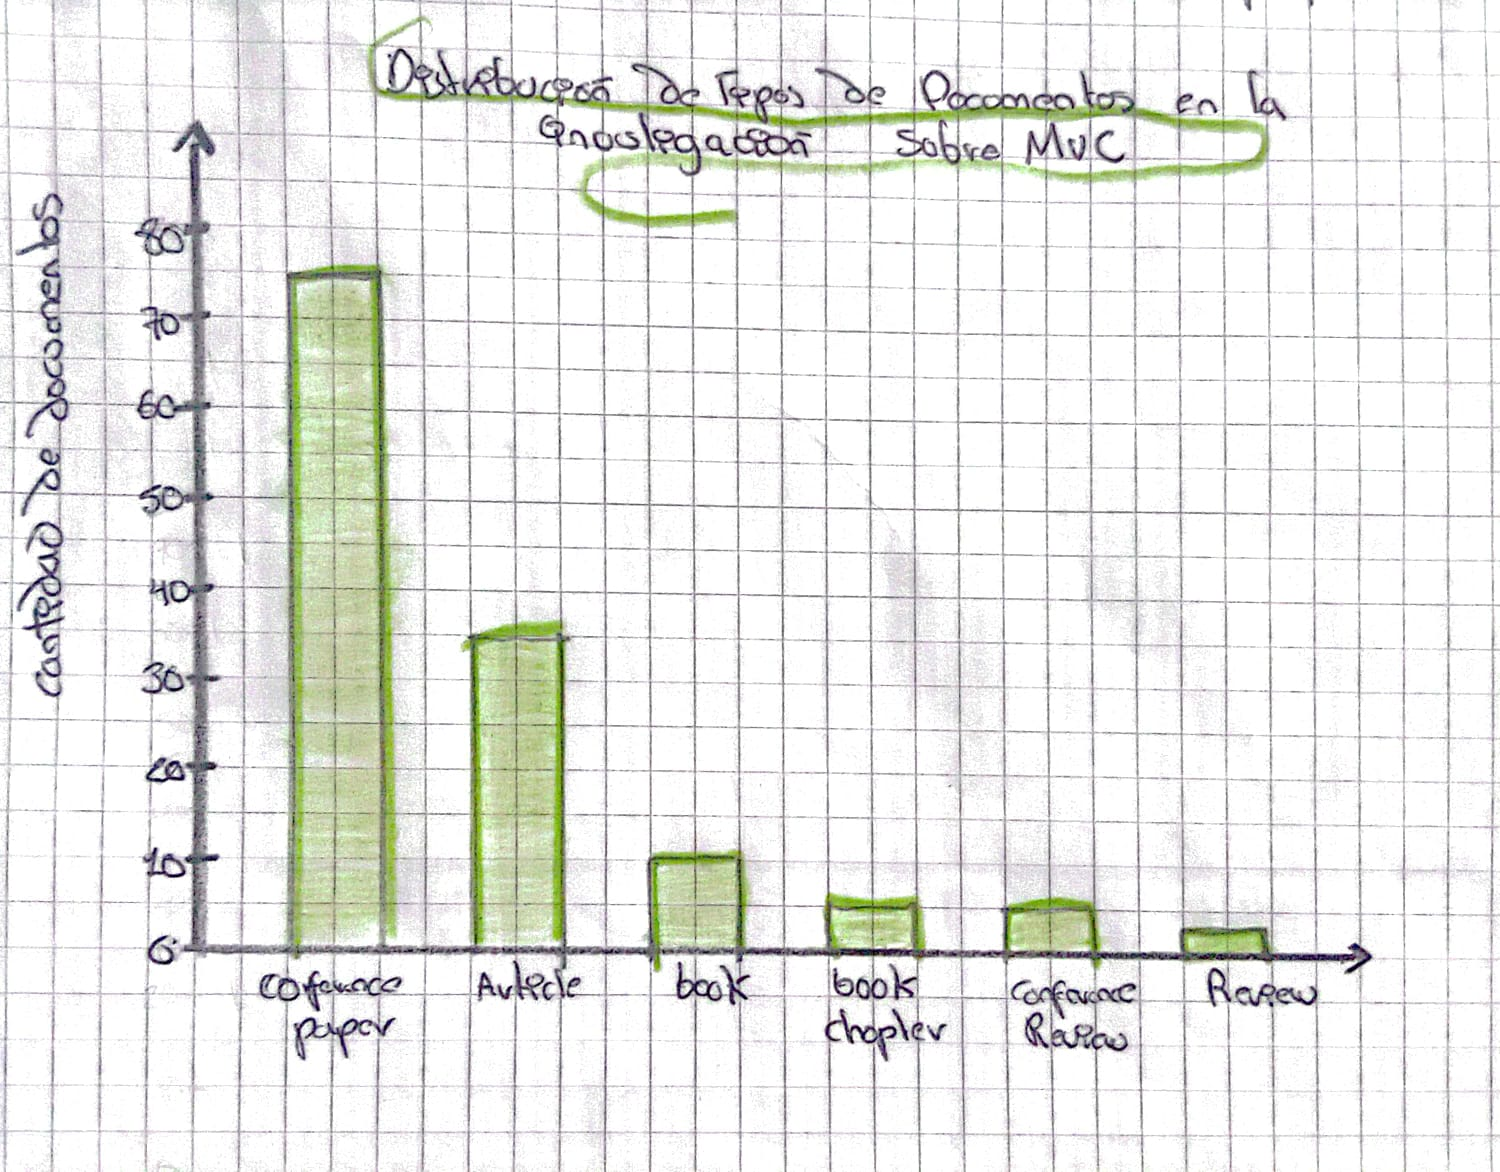
\includegraphics[width=0.5\textwidth]{graphics/Grafica1.jpeg}
\caption{Gráfica de apoyo 1}
\label{fig:grafica1}
\end{figure}

\begin{figure}[h]
\centering
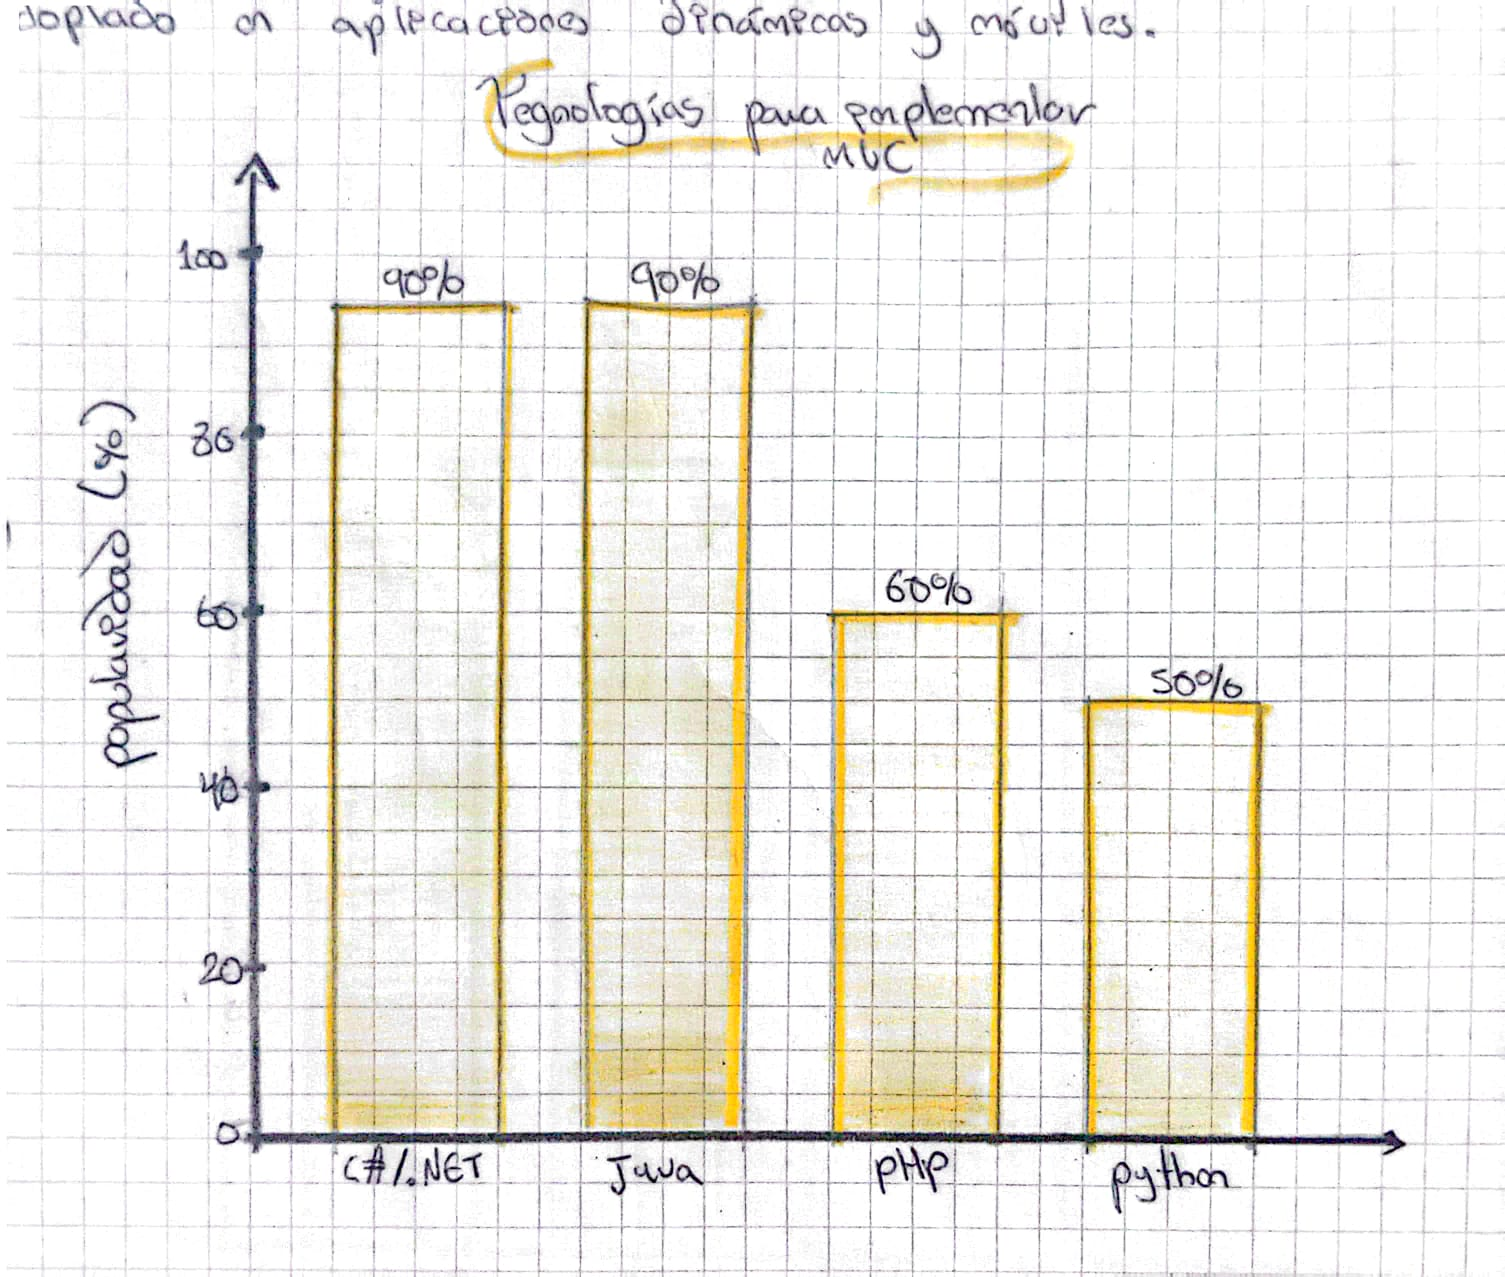
\includegraphics[width=0.5\textwidth]{graphics/Grafica2.jpeg}
\caption{Gráfica de apoyo 2}
\label{fig:grafica2}
\end{figure}

\subsection{Ejemplo de Clase Controller}
\begin{lstlisting}[language=Java, caption=Ejemplo de Controller en Spring Boot]
@RestController
@RequestMapping("/api/events")
public class EventController {

    @Autowired
    private EventService eventService;

    @GetMapping
    public ResponseEntity<ResponseDto<List<EventDto>>> getAllEvents() {
        List<EventDto> events = eventService.getAllEvents();
        return ResponseEntity.ok(new ResponseDto<>(events, "Events retrieved successfully"));
    }

    @PostMapping
    public ResponseEntity<ResponseDto<EventDto>> createEvent(@RequestBody EventDto eventDto) {
        EventDto createdEvent = eventService.createEvent(eventDto);
        return ResponseEntity.status(HttpStatus.CREATED)
                .body(new ResponseDto<>(createdEvent, "Event created successfully"));
    }
}
\end{lstlisting}

\subsection{Ejemplo de Componente React}
\begin{lstlisting}[language=JavaScript, caption=Componente de Lista de Eventos en React]
import React, { useState, useEffect } from 'react';
import axios from 'axios';

const EventsList = () => {
    const [events, setEvents] = useState([]);
    const [loading, setLoading] = useState(true);

    useEffect(() => {
        const fetchEvents = async () => {
            try {
                const response = await axios.get('/api/events');
                setEvents(response.data.data);
            } catch (error) {
                console.error('Error fetching events:', error);
            } finally {
                setLoading(false);
            }
        };

        fetchEvents();
    }, []);

    if (loading) return <div>Loading...</div>;

    return (
        <div className="events-list">
            {events.map(event => (
                <div key={event.id} className="event-card">
                    <h3>{event.eventName}</h3>
                    <p>{event.description}</p>
                    <p>{event.startDate}</p>
                </div>
            ))}
        </div>
    );
};

export default EventsList;
\end{lstlisting}

\subsection{Métricas Detalladas}
Tabla completa de métricas para todas las clases evaluadas (ver Sección 5 para resúmenes).

\subsection{Código Fuente Completo}
El código fuente completo de TuEvento está disponible en el repositorio del proyecto. Para acceso, contactar a los autores.